\section{Classification}
\label{section:data_classification}

The next task was to analyse the data selected for use in the development and training of a model and then classify each questions as either bullying or not bullying. As described in Chapter \ref{chapter3}, cyberbullying can take many forms such as flaming, outing, exclusion, flooding, cyberstalking, impersonation or masquerading, trolling and denigration of their victims. These attacks could then be categorised as sexual, racial, cultural or against the intelligence or physical appearance of a person or their socio-economic status to name but a few. The types and categories of cyberbullying are further examined and analysed to develop a sense of the criteria against which to evaluate each question. Once evaluated, each question will then be classified as bullying or not bullying.

\subsection{Cyberbullying Criteria}

This section provides more details about the type of on-line post, or in this case question, that should be considered as cyberbullying.

\textit{``Flaming''} is usually considered as off topic insults or attacks against an individual or group and are more typically seen in a bulletin board or discussion type forums. A classic example of flaming is where a discussion comparing the virtues of the Linux, Microsoft Windows and Apple Mac operating systems disintegrates into a series of posts where each side questions the intelligence of the other two groups for using such an obviously inferior product. In the context of the ask.fm dataset, it is unlikely that a series of posts of this type would be obviously detectable. The nature of the question and answer format, the order of the answers given, and their intermingling with other question would prevent it. Some questions that are obviously flaming made even be deleted or blocked. However, even if a series of questions that are flaming in their nature, either against an individual or a number of individuals, cannot be specifically identified as flaming their hostility, aggressiveness or derogatory sentiments would probably guarantee that they are identified as bullying. A user that purposefully starts, encourages or engages in such flaming activities is sometimes known as a \textit{``Troll''} and by denigrating or annoying people in this manner they are said to be \textit{``Trolling''}

The  term \textit{``outing''} is typically used to describe the disclosure of a persons sexual orientation, for example, revealing for the first time that a person is gay. As the users of the Ask.fm site are mostly teenagers and young adolescents, and because of the amount of sarcasm and black humour observed, it would be difficult reading isolated questions to determine whether a genuine outing has occurred. There is no facility to validate any such outing claim, or to determine if the question is just a slanderous attack. Regardless of these uncertainties, any post that appears to out someone or to question their sexual orientation must be considered as bullying.

Cyber \textit{``exclusion''} can be considered as any type of activity that purposefully excludes an individual or group from an event, a party, shopping trip or holiday, for example.  Alternatively, perhaps, they are prevented from joining a sports team or social group. This exclusion could take the form of inviting everyone to a party but then, explicitly, uninviting the excluded person in a public and humiliating manner. Another scenario could be to openly mock or taunt someone because they were prevented from joining a popular social clique in school. Any such obvious exclusionary activity seen in the Ask.fm dataset would be highlighted as bullying.

In some ways \textit{``flooding''} could be seen as similar in nature to a Denial of Service (DoS) attack on a website. A DoS attack is an attempt to interrupt the normal functioning of a website or make it unavailable to users by bombarding the site with so many requests that the sites response time to legitimate traffic is extremely slow or non-existent, rendering the site unusable. In a chat room, flooding could be seen as repeatedly, and in very quick succession, posting empty messages or the same message again and again to prevent other users in the chat room from voicing their opinion. Alternatively, in the context of the Ask.fm dataset, flooding could be considered as the repeated asking of the same question or requests for information. Such flooding activity, if seen, should be considered bullying. However, as the data has been both anonymised and randomised, or instances of flooding may already have been deleted by the targeted user, it may be difficult to identify.

Stalking is seen as the unwanted, obsessive and criminal intrusion into the personal life of an individual by another person. When computers or other electronic equipment is used it can be considered as \textit{``cyberstalking''}. The actions of a stalker can include activities such as a desire to control their victim, to subversively gather information about them, monitoring and anonymously commenting on their on-line activity and making claims of false victimisation against the target and  other false accusations such as defamation and libel. Other behaviours exhibited by the stalker may include flooding the victims with constant requests for personal information or for requests to meet in person. Any questions that are malicious in nature, from their content or tone, should be considered bullying. However, some questions, which may at first appear innocuous, for example ``how old are you'', ``where were you last night'' or ``send me a selfie'' should also be classified as bullying as they are requesting personal information which could be used by a potential stalker.

\textit{``Impersonation''} or \textit{``Masquerading''} is where a person creates a false identity, or assumes the identity of someone else, when posting or creating on-line content. Typically the reason for posting content using this assumed or false identity is to harm the reputation of the person they are pretending to be, by making what appear to be personally humiliating comments or by making harmful, harassing, confrontational or bullying remarks against another person. Alternatively the owner of a false account could  use it solely for the purpose of anonymously posting harmful content while observing on-line etiquette with their real name account. Due to the anonymous nature of the content on the Ask.fm site and the lack of any validation of a persons true identity it would be difficult if not impossible to ascertain whether a question is asked by a user masquerading or impersonating another person. However, it could also be argued that regardless of who posted the question if it meets any of the criteria that identify cyberbullying then it should be marked as such.

It is also important to consider the tone and content of a cyberbullying incident as well as the various forms that it may take. As well as threats of physical violence, the wishing of harm on a person, or by goading a perform to harm themselves, the tone of a cyberbullying attack can be categorised in many ways including gender, sexist, racial, cultural, nationality, ethnicity, colour or race, intellectual, appearance, religious or socio-economic. Questions that could be considered confrontational, libellous, defamatory or make unfounded accusations that are intended to be hurtful or that could result in unstated repercussions should be considered as bullying. 

Gender or sexist attacks would typically target women or sexual minorities, for example gay, lesbian, bisexual or transgender orientation. Simple examples of this type of cyberbullying would be name calling such as referring to a person as a \textit{``bitch''}, \textit{``faggot''} or \textit{``dyke''} or questions relating to sexual experience. Other more sinister types of these attacks would include unwanted sexual advances or invitations to engage in or descriptions of unsolicited sexual activity. An extreme case would be the threat or implication of rape. Racial or cultural bullying includes slurs or attacks against a cultural minority and its traditions, or direct attacks against a person based solely on their skin colour, ethnicity, race or nationality. Questions asking someone in a derogatory way if they are mentally or physically handicapped or questions that are hurtful or mean about their weight, height or general appearance are all bullying.

Though difficult to identify in isolation, text that may be considered grooming in nature should also be identified. There are multiple different categories of grooming approaches including Approach, Communicative Desensitisation, Compliment, Isolation and Reframing. Samples of each type of categories are \textit{``i just want to meet''}, \textit{``how cum''}, \textit{``you are a really cute girl''}, \textit{``are you alone''} and \textit{``let's have fun together''}  \cite{kontostathis_chatcoder:_2009}

It should be noted that profanity, without any of the other criteria listed here, would not, for the purposes of this research, be considered as cyberbullying.

The criteria for identifying cyberbullying can be summarised as follows:

\begin{enumerate}

	\item Can readily be identified as being attempts at flaming or of flooding.
	\item Is an obvious attempt to exclude or isolate an individual from a group or event.
	\item Could be perceived as stalking by overtly asking for personal information or photos 
	\item May be considered grooming where the question could be seen as an approach, an attempt to isolate or any of the other categories defined.
	\item Unnecessarily sexually explicit references or unsolicited invitations or by outing an individual whether real or perceived.
	\item Derogatory comments about race, culture, nationality, ethnicity or religion.

\end{enumerate}

\subsection{Dataset Classification}
Once the criteria to be used to identify a question as bullying had been determined the next step was to classify the block of questions that were to be used to train and test the initial model. Classification was a two step process. First all questions were reviewed and classified as either bullying, not bullying or discard. In total 10,914 question were reviewed. 1,644 were classified as bullying, 78 were classified as discard and the remainder as not bullying. Questions that were classified as discard contained only digits, emoticons or what appeared to be random characters. 

To validate that the classification criteria specified are both meaningful and understandable and that the original classification was repeatable, accurate and consistent, a random selection of 500 questions, 250 bullying and 250 not bullying, were independently classified by two other reviewers. Each reviewer was given the classification criteria described here and a print out of the original unedited questions. They were then asked to classify each sample question as either bullying or not bullying. The results from each reviewer is shown in Figure \ref{fig:chapter4:reviewer_results}

\begin{figure}[htbp]
	\centering
	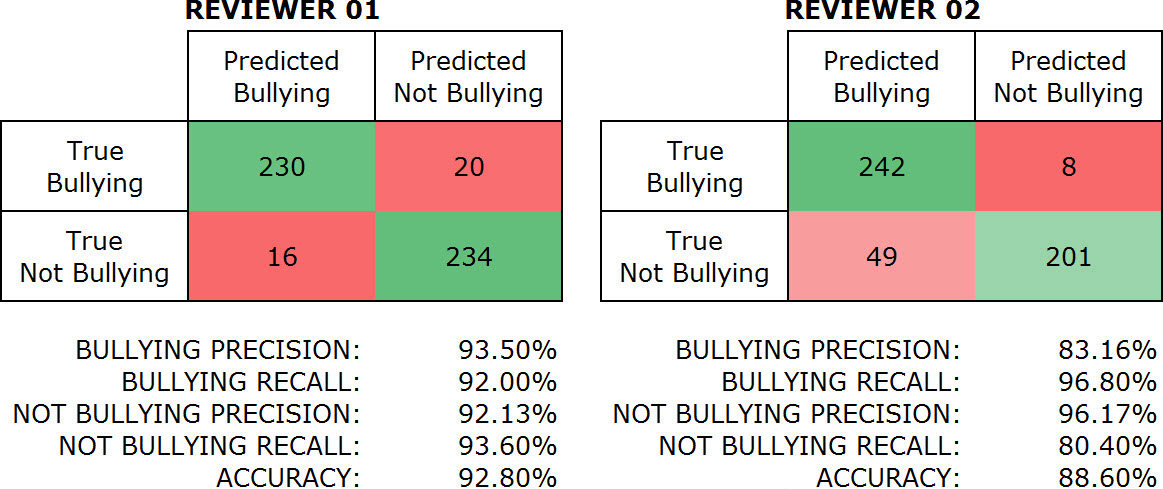
\includegraphics[width=0.9\textwidth]{Figures/Chapter4/reviewer_results.jpg}
	\caption[Independent classification review results]{Matrix showing the number of questions classified as bullying and as not bullying by two independent reviewers}
	\label{fig:chapter4:reviewer_results}
\end{figure}

In total, the first reviewer classified 246 questions as bullying of which 230 were originally identified as bullying. The second reviewer predicted 291 questions as bullying, of which 242 were originally identified as bullying. In total 224 of 250 sample questions, or just under 90\%, were identified by all three classifiers as bullying. However, 248 out of 250 sample bullying questions, or 99.2\%, were identified as bullying by two out of the three classifiers. Of note, 14 sample questions, that were originally classified as not bullying, were classified as bullying by both the independent reviewers. At just over 5.5\% this is not hugely significant but important to highlight. Overall, however, this was a very satisfactory validation of the both the classification criteria and the original classification of the complete dataset.

Before leaving this section, it is worth briefly examining some of the questions that were classified as bullying and understand why they were so classified. All the samples listed here are genuine examples from the Ask.fm dataset that was classified. Some of the samples have been abbreviated so as to highlight the relevant part of the question.

\begin{itemize}

	\item Asking someone their age. \\
	Asking how old they are could be very innocent and a genuine friendly request. However, it could just as easily be considered as stalking or as grooming. 
		\begin{itemize}
			\item \verb|Age?|
			\item \verb|How old are you?| 
		\end{itemize}
		
	\item Asking for information of an obviously private nature
		\begin{itemize}
			\item \verb|What Bra size are you?|
			\item \verb|can i have ur number?|
			\item \verb|How many ladies have you slept with?|
		\end{itemize} 

	\item Asking someone to post a picture or video of themselves often requesting specific parts of the body, clothes or naked.
		\begin{itemize}
			\item \verb|Puberty progress photo?|
			\item \verb|bikini picture?|
			\item \verb|Pap of you right now?|
		\end{itemize}

	\item Asking someone about their sexual experience or preferences
		\begin{itemize}
			\item \verb|Are you a virgin?|
			\item \verb|Are you good at giving head ?|
			\item \verb|butt or boobs|
		\end{itemize}
	
	\item Threatening physical violence or goading others to hurt themselves
		\begin{itemize}
			\item \dots \verb|Cut your self ugly saggy ass hoe|
			\item \dots \verb|I'm gonna beat your trashy little twig of an ass in so far| \\ \verb|     you'll puke it out| \dots
			\item \dots \verb|i will slap you across your f**king mouths|
		\end{itemize}

\end{itemize}

Before leaving this section it is important to note that these are only a small example of the questions that were classified as bullying. The content of a large proportion of the question would be considered crude, vulgar and too offensive to list here.